\documentclass[12pt,a4paper]{article}
\usepackage[utf8]{inputenc}
\usepackage{amsmath}
\usepackage{amsfonts}
\usepackage{amssymb}
\usepackage{graphicx}
\usepackage[left=2cm,right=2cm,top=2cm,bottom=2cm]{geometry}
\author{leonardo}
\title{diagrama electrico de interfaz de potencia }
\begin{document}
\section{Introduccion}
\begin{flushleft}
Las redes resistivas tienen la desventaja de depender en gran medida de las características específicas de
disparo de cada tiristor.
El nivel de potencia en el circuito de control es alto debido a que toda su corriente debe fluir a través de
resistencias.
La corriente de disparo sigue la forma de onda senoidal del voltaje de alimentación.
El disparo de tiristores mediante pulsos de corriente puede adaptarse a tolerancias
amplias en las características de disparo.
Debido a que este ataque en corriente en corriente a la compuerta la hace sobreconducir, garantizando el
cebado de cualquier tiristor.
Se han desarrollado diversos dispositivos de disparo que generan los pulsos de corriente de puerta
necesarios para cebar un tiristor.
Existen dispositivos de disparo unilateral y bilateral, encontrándose entre ellos el DIAC.
Diac
El Diac es un diodo bidireccional de disparo y es un elemento ideal en circuitos de control de puerta el
triac.
Proporciona pulsos de corriente a la compuerta del tiristor garantizando su cebado independientemente de
sus características de disparo.
Por ser un elemento bidireccional, permite el cebado del triac en ambas polaridades, concretamente en los
cuadrantes 1y 3 La figura 1 muestra la estructura de capas p y n, el símbolo del circuito y la curva
característica voltaje – corriente del Diac.
De la curva característica se observa que para voltajes positivos menores que el voltaje de ruptura directo
(+vbo), el Diac prácticamente no permite el flujo de corriente.
Una vez que el Diac alcanza el voltaje de ruptura directo conmuta a conducción y la corriente aumenta
rápidamente a la vez que el voltaje entre terminales disminuye.
El súbito aumento de corriente explica la habilidad del Diac para producir pulsos de corriente.
En la región de voltaje negativo, la operación es idéntica.
Cuando el voltaje inverso es menor (en realidad mayor, más positivo) que el voltaje inverso de ruptura (-
vbo), el Diac impide el flujo de corriente.
Cuando el voltaje aplicado alcanza –vbo, el Diac conmuta a conducción en la dirección opuesta
produciéndose un pulso de corriente negativa.
Los Diacs son relativamente estables con la temperatura y presentan una pequeña tolerancia entre los
voltajes de ruptura directo e inverso, siendo la diferencia típica entre ellos de menor a 1 volt.
Lo anterior permite que el circuito de disparo mantenga prácticamente iguales los ángulos de disparo en
ambos semiciclos del voltaje alterno de alimentación.
Otra observación sobre la curva, es que exhibe una característica de resistencia negativa más allá de la
corriente de ruptura (ibo) en ambas polaridades, que se extiende hacia todo el rango de operación de
corrientes una vez superada esta corriente de ruptura.
\end{flushleft}
\begin{flushleft}
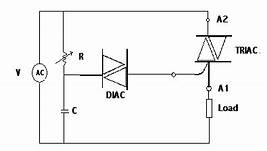
\includegraphics[width=10cm]{1.jpg} 
\end{flushleft}
\section{materiales}

\begin{flushleft}
1.-transformador
\end{flushleft}
\begin{flushleft}
2.-bobina
\end{flushleft}
\begin{flushleft}
3.-capacitores
\end{flushleft}
\begin{flushleft}
4.-resistor
\end{flushleft}
\begin{flushleft}
5.-triac
\end{flushleft}
\begin{flushleft}
6.-diac
\end{flushleft}
\section{Funcion}

\begin{flushleft}
 Se emplea normalmente en circuitos que realizan un control de fase de la corriente del triac, de forma que solo se aplica tensión a la carga durante una fracción de ciclo de la alterna. Estos sistemas se utilizan para el control de iluminación con intensidad variable, calefacción eléctrica con regulación de temperatura y algunos controles de velocidad de motores.
 La forma más simple de utilizar estos controles es empleando el circuito representado en la Figura 3, en que la resistencia variable R carga el condensador C hasta que se alcanza la tensión de disparo del DIAC, produciéndose a través de él la descarga de C, cuya corriente alcanza la puerta del TRIAC y le pone en conducción. Este mecanismo se produce una vez en el semiciclo positivo y otra en el negativo. El momento del disparo podrá ser ajustado con el valor de R variando como consecuencia el tiempo de conducción del TRIAC y, por tanto, el valor de la tensión media aplicada a la carga, obteniéndose un simple pero eficaz control de potencia
\end{flushleft}
\section{Conclusion}
\begin{flushleft}
en la practica note que el la bobina que hice influye puesto que al enbobinarla con otros dos cables vi que la pila alimentaba 3 leds al incorporar el enbobinado que hicimos bajo punto 3 decimas
\end{flushleft}


\end{document}